    \chapter{Comparativo Android x iOS} \label{CHP:COMP}%%
    \section {Ambientação}
     
    \subsection{iOS}
    
	Para implementação nativa de aplicações, utilizamos a \ac{IDE} gratuita chamada \emph{Xcode}. Desenvolvida pela Apple Inc., funciona apenas sobre o sistema operacional \emph{Mac OS X}.  Por padrão, já vem com suporte ao Objective-C, linguagem de programação utilizada para desenvolvimento de aplicativos nativos no \emph{Mac OS X} e no \emph{iOS}.
    
	Atualmente, o \emph{Xcode} está na versão 4.5.2 e pode ser baixado via Mac App Store, de forma gratuita para usuários do \emph{Mac OS X Lion} e \emph{Mac OS X Mountain Lion}, disponível em \cite{xcode}.
    
	Para desenvolvimento \emph{iOS}, é necessário possuir o \emph{iOS SDK}, que pode ser baixado internamente a ferramenta \emph{Xcode}. Entretanto, para realização de testes no dispositivo, é necessária a posse da licença de desenvolvimento.
     
    \subsection{Android}
           
		    Para o desenvolvimento de aplicações nativas em \emph{Android}, necessita-se de um ambiente que possua \emph{Android SDK} instalado. É possível, por exemplo, gerar aplicativos utilizando apenas um editor de texto, como Notepad ou Gedit. Entretanto, a Google recomenda o uso do Eclipse com ADT Plugin, disponível em \cite{adt}.
           
     
    %\subsection{IDEs}
   % \section {Arquitetura}
    %\subsection {Arquivos gerados}
     
     

    \section {Mostrando textos}
    \subsection{iOS}
    
	Para exibir textos sem interação direta com o usuário, utilizamos uma instância da classe \texttt{UILabel}. Essa classe possui algumas propriedades para modificação de aspectos, a saber:
\begin{itemize}
\item \texttt{text}: o texto mostrado no campo;
\item \texttt{textColor}: cor do texto;
\item \texttt{numberOfLines}: número máximo de linhas suportadas;
\item \texttt{font}: fonte utilizada pelo texto, instância de \texttt{UIFont}.
\end{itemize}     
   
    \subsection{Android}
     
    De maneira similar ao \emph{iOS}, o \emph{Android} possui um controle específico para mostrar textos na tela, chamado \texttt{TextView}. Um \texttt{TextView} pode ser definido no \emph{layout} \ac{XML} ou no próprio Java. Assim como no \emph{iOS}, possui uma propriedade do tipo \texttt{String} chamada ``text'', a qual representa o texto apresentado.% Possui também algumas propriedades, a saber:
    
	%[as propriedades legais]
   
    Uma diferença importante entre o \texttt{UILabel} e o \texttt{TextView} é que o último aceita interações com o usuário; podemos colocar eventos de interação com o usuário. Essa funcionalidade costuma ser usada com textos que representam \emph{links}.
     
    \section {Inserindo textos}
     
    \subsection{iOS}
            Para entrada de textos, utilizamos uma instância de \texttt{UITextField}. A manipulação do texto é feita através do disparo de uma ação para um \emph{target} quando o usuário pressiona o botão \emph{return} do teclado.
    
	Essa classe normalmente é associada a um \texttt{UITextFieldDelegate}, o qual fornece métodos adicionais de decisão.
    
	Quando o usuário toca em um \texttt{textfield}, esse controle torna-se o \emph{first responder} e invoca o aparecimento do teclado para o sistema. O teclado deve ser configurado, pelo desenvolvedor, para desaparecer quando o botão de \emph{return} for pressionado. Isso deve ser feito através da mensagem \texttt{resignFirstResponder}, a ser enviada para o \texttt{textfield}.
    
	Para que o \texttt{textfield} não fique ``escondido'' na tela, embaixo do teclado, cabe ao desenvolvedor mover tela de maneira conveniente, de forma a aparecer o conteúdo.
   
    A aparência do teclado pode ser configurada utilizando o protocolo \texttt{UITextInputTraits}. Existem, entretanto, alguns tipos de teclado a serem definidos por padrão, como o \emph{ASCII, Number, Url, Email,} entre outros.
     
    \subsection{Android}
     
    Para a entrada de texto do usuário, o Android fornece o controle chamado \texttt{EditText}. Assim como o \texttt{UITextField}, esse controle possui uma propriedade chamada \emph{text}, que representa o texto mostrado no controle. Esse texto pode ser tanto a entrada do usuário como também um texto configurado via programação pelo aplicativo.
    
	%O EditText possui algumas propriedades que usamos na aplicação, como as seguintes:
    
	%[propriedades legais]
    
	Para cada \texttt{EditText}, podemos definir o tipo de teclado que será exibido ao interagir com o usuário, como teclados de telefone, números e de letras.
    
	O \texttt{EditText} possui duas grandes diferenças em relação ao \texttt{UITextField}, a saber:
\begin{itemize}
	\item O teclado retorna automaticamente quando terminada a edição;
	\item Ao entrar em modo de edição, o \texttt{EditText} faz com que a tela do aplicativo desloque-se, caso seja necessário para aparecer o conteúdo do controle.
\end{itemize}     
     
    \section {Botões e eventos}
     
    \subsection{iOS}
           
    Um botão é representado por uma instância da classe \texttt{UIButton}. Os botões interceptam eventos de toque e enviam mensagens para um \emph{target}(alvo) pré-definido quando tocados. Métodos para configurar os \emph{targets} e ações são herdados de \texttt{UIControl}. Como atributos, possuem título, imagem e outras propriedades de aparência.
     
     
    Os botões respondem a algumas ações, como \texttt{touch drag, touch down, touch up,} entre outros. Para associar um método a um evento, criamos uma \texttt{IBAction} (método) e, ao evento, indicamos tal \texttt{IBAction}. Isso pode ser feito facilmente no \emph{Interface Builder/Xcode}, ``ligando'' o botão ao código correspondente (\emph{file's owner} desse botão), conforme os passos abaixo:
\begin{enumerate}     
\item Arrastar, com o botão direito, o botão ao código do \emph{file's owner}
		 \begin{figure}[H]
		   % Requires \usepackage{graphicx}
		   \centering
		   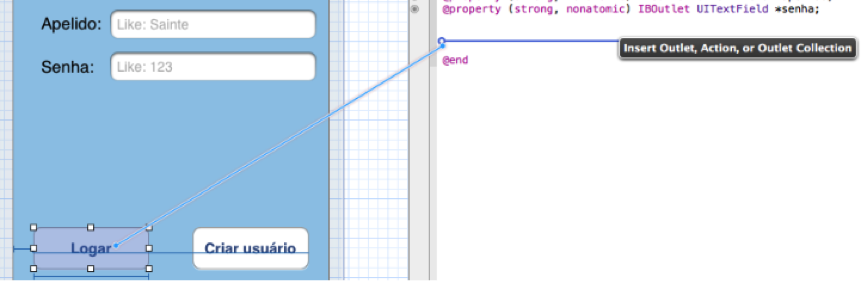
\includegraphics{figs/iosbtn1.png}\\
		   \caption{ Criando ligação entre interface builder e o código }
		   \label{FIG:iosbtn1}
		 \end{figure}
         
 \item Nomear um \texttt{IBAction} e associar um evento
 \begin{figure}[H]
   % Requires \usepackage{graphicx}
   \centering
   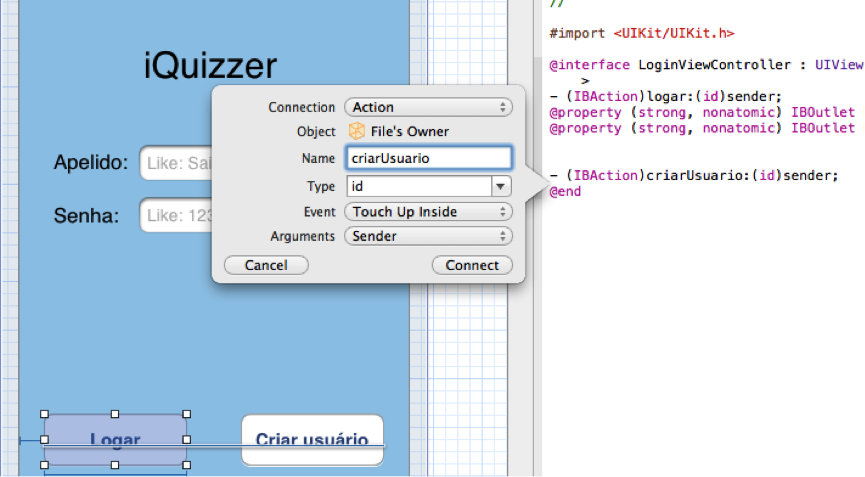
\includegraphics{figs/iosbtn2.png}\\
   \caption{ Criando IBAction e associando evento }
   \label{FIG:iosbtn2}
 \end{figure}
 
 \end{enumerate}    
     
    \subsection{Android}
     
    Os botões no \emph{Android} pertencem à classe \texttt{Button}. Existem duas formas de inserir eventos nos botões, a saber:
\begin{itemize}
\item via \texttt{Listener} Java: podemos implementar o \texttt{OnClickListener} na \texttt{Activity} ou em alguma classe anônima dentro da \texttt{Activity}, de modo que ao disparar o evento de \emph{click}, o método \texttt{onClick()} da interface seja chamado.
\item via propriedade \texttt{onClick} no \texttt{LayoutXML}: os botões possuem uma propriedade chamada \texttt{onClick}, que recebem uma \texttt{String} como valor. Esse valor é o nome do método da \texttt{Activity} onde o \emph{layout} contendo esse botão foi inflado\footnote{Para que um \emph{layout} \ac{XML} ser colocado dentro de outro \emph{layout} \ac{XML}, é necessário ``inflar'', utilizando a classe \texttt{LayoutInflate}.}.
    Neste projeto, foi utilizado somente \texttt{onClick} como propriedade \ac{XML}, uma vez que toda a parte de \emph{layout} foi implementada via \ac{XML}.
\end{itemize}    
    \section {Criando listas}
    \subsection{iOS}
     
    Listas em \emph{iOS} são feitas utilizando instâncias de \texttt{UITableView}. Essa classe, por sua vez, estende de \texttt{UIScrollView}, que habilita a rolagem vertical (e apenas a vertical). Internamente, cada linha (célula) é representada por um objeto de \texttt{UITableViewCell}, que são totalmente configuráveis.
    
	Esse controle normalmente é associado a um \texttt{UINavigationController}: quando uma célula é tocada, é feito um \emph{push} de um novo \texttt{UIViewController}, detalhando a célula.
    
	\emph{Table views} possuem dois estilos, a saber: \texttt{UITableViewStylePlain} e \texttt{UITableViewGrouped}. Uma vez criado o controle, não é possível mudar o estilo. No estilo \texttt{Plain}, as seções de \emph{header/footer} flutuam nas bordas do conteúdo. Nesse estilo, pode haver um índice variando de A - Z, que facilita a navegação vertical. No estilo \texttt{Grouped}, uma cor padrão é definida para o fundo da \emph{view} e das células. Nesse estilo, podem ser criadas várias listas, de formas agrupadas. Nesse caso, não podem ter índice.
    
	Muitos métodos utilizam o objeto do tipo \texttt{NSIndexPath} como parâmetro e retornam valores. Esse objeto representa o índice da linha atual e da seção atual.
    
	Um objeto do tipo \emph{Table View} necessita de um objeto que atue como fonte de dados (\emph{data source}) e um objeto que atue como \emph{delegate}. Normalmente, utilizamos os protocolos \texttt{UITableViewDataSource} e \texttt{UITableViewDelegate} no \texttt{UIController} no qual o \emph{table view} esteja inserido. O \emph{data source} fornece informação que o \texttt{UITableView} precisa para construir tabelas e o \emph{delegate} fornece as células e executa alguns outros métodos de manipulação.
    
	A fim de criar uma \emph{table view} básica, precisa-se implementar, no mínimo, os seguintes métodos \emph{data source}:
\begin{enumerate}
\item Número de seções - retorna o número de seções para essa \emph{table view}

\begin{lstlisting}[language=C]   
-(NSInteger)numberOfSectionsInTableView:(UITableView *)tableView;
\end{lstlisting}   
	   
\item Número de \emph{rows} (linhas): retorna o número de linhas para cada uma das seções

\begin{lstlisting}  
- (NSInteger)tableView:(UITableView *)tableView
 numberOfRowsInSection:(NSInteger)section;  
\end{lstlisting}  
   
\item \emph{cell for row at index}: define uma célula para cada \emph{index} (par linha/seção) da tabela
\begin{lstlisting}    
-(UITableViewCell *)tableView:(UITableView *)tableView
 cellForRowAtIndexPath:(NSIndexPath *)indexPath;
     
\end{lstlisting}

\end{enumerate} 

    Além desses métodos, é comum implementar um método \emph{delegate} que responda a cada célula tocada, como a seguir:
 
    \emph{did select row at index}: informa o par (linha/seção) que foi selecionado. A partir do \emph{index path}, pode-se recuperar a célula selecionada dentro da \emph{table view}
\begin{lstlisting}
- (NSInteger)tableView:(UITableView *)tableView 
didSelectRowAtIndexPath:(NSIndexPath*)indexPath;  
\end{lstlisting}   
     
    Para a tela de escolha dos \emph{quizzes} (\texttt{GameMenu}), implementou-se uma \emph{table view} simples, da seguinte maneira:
\begin{lstlisting}[language=C]  
-(NSInteger)numberOfSectionsInTableView:(UITableView *)tableView{
    return 1;
}
-(NSInteger)tableView:(UITableView *)tableView
	 numberOfRowsInSection:(NSInteger)section{
    //conta no array de quizzes a quantidade de elementos
    return [self.quizzes count];
}

-(UITableViewCell*)tableView:(UITableView *)tableView
 cellForRowAtIndexPath:(NSIndexPath *)indexPath{
    /* reaproveita ou cria uma célula*/
    UITableViewCell* cell = 
    [tableView dequeueReusableCellWithIdentifier:@"cell"];
	
    if (cell == nil){
        cell = [[UITableViewCellalloc] init];
    }
     
    /* personalizacao da celula */
    Quiz* q = [self.quizzesobjectAtIndex:indexPath.row];
    cell.textLabel.text = [q titulo];
	
    return cell;
}

/* disparado quando um dos quizzes for selecionado */
-(void)tableView:(UITableView *)tableView
 didSelectRowAtIndexPath:(NSIndexPath *)indexPath{
    Quiz* q = [self.quizzesobjectAtIndex:indexPath.row];
    GameViewController* gq = [[GameViewController alloc] 
	initWithNibName:@"GameViewController" bundle:nil];
    
	gq.quiz = q;
	
	//navegando entre telas
    [self.navigationController pushViewController:gq animated:YES];
}
\end{lstlisting} 
   
    \subsection{Android}
            
			As listas em \emph{Android} são instâncias da classe \texttt{widget ListView} e, assim como no \emph{iOS}, já possui rolagem vertical implementada. Os itens da lista são inseridos por outra classe controladora, chamada \texttt{Adapter}.
            
			O \texttt{Adapter} é uma classe que provê acesso aos itens que contém a informação, como um \texttt{array} de \texttt{strings}. Além disso, o \texttt{Adapter} é responsável por criar o \emph{layout} de cada célula.
           
		    Para a lista simples mostrada em \texttt{GameMenu}, foi implementado uma lista com células padrão da seguinte maneira:
\begin{lstlisting}[language=Java,frame=single,breaklines=true]   
private void carregarLista() {
     
    ArrayAdapter arrayAdapter = new ArrayAdapter(this,
	 android.R.layout.simple_list_item_1, quizzes);
    ListView listView = (ListView)findViewById(R.id.lista_quizzes);
    listView.setAdapter(arrayAdapter);
    listView.setOnItemClickListener(this);
     
}
\end{lstlisting} 

	Nesse trecho de código, \emph{quizzes} é um \texttt{ArrayList} de \emph{quizzes}. \texttt{ArrayAdapter} e \texttt{ListView} são classes padrão do \emph{Android}.  
    
	Os eventos de clique de célula estão associados a classe que implementa a interface \texttt{OnItemClickListener}.  Tal interface exige a implementação do método \texttt{onClickListener()}. Foi utilizado, no iQuizzer, esse \emph{listener} na classe \texttt{GameMenu}, tendo sido implementado o método da seguinte maneira:
\begin{lstlisting}[language=Java]   
@Override
public void onItemClick(AdapterView<?> adapterView, View view,
 int position, long id) {
    Quiz quiz = quizzes.get(position);
    Intent i = new Intent(getApplicationContext(), GameActivity.class);
    i.putExtra("quiz",quiz);
    startActivity(i);
}
             \end{lstlisting}    
    %\section{Personalizando linhas de uma lista} -- retirado
    %iOS
    %Android
    \section {Acesso a dados}
     
    \subsection {SQLite}
	
            O  SQLite é uma biblioteca implementada em C, de domínio público, que representa um banco de dados SQL. Tem como características fundamentais ser contido em si mesmo, livre de servidores, sem configuração e transacional, conforme descrito em \cite{SQLite}.
            
			Tanto o \emph{iOS} quanto o \emph{Android} possuem abstrações para representar objetos da tabela (\emph{active records}), conexões e o próprio banco.
     
    \subsubsection{iOS}
            Existem duas maneiras de se trabalhar com SQLite em \emph{iOS}: acesso nativo através da biblioteca \texttt{SQLite.h} e \texttt{Core Data Framework}.
           
		    No acesso nativo, a programação utilizada é a mesma para aplicações nativas em C, ou seja, não há particularidades entre utilizar o SQLite dentro ou fora do iOS. Já em \texttt{Core Data}, a programação é em Objective-C e existe uma camada de abstração do banco de dados.
           
		    Na aplicação, optou-se por usar o \texttt{Core Data} devido à facilidade de fazer a modelagem utilizando o \emph{xcdatamodel}. O \emph{xcdatamodel} é uma ferramenta facilitadora, integrada ao \emph{Xcode}, na qual o desenvolvedor pode ``desenhar'' as tabelas e criar ligações, chamadas \emph{relationships}. Cada uma das tabelas e relações possui propriedades, que são facilmente configuradas.
     
	 \begin{figure}[H]
	   % Requires \usepackage{graphicx}
	   \centering
	   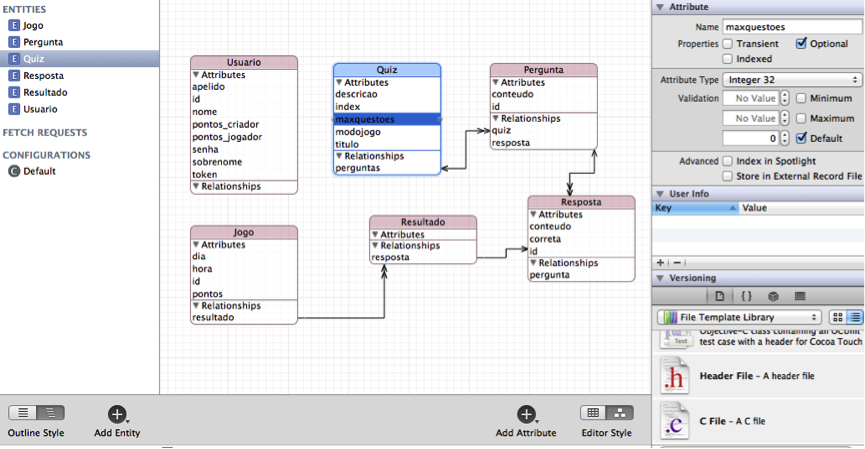
\includegraphics{figs/iosmanaged.png}\\
	   \caption{ Ferramenta gráfica para manipulação do banco de dados utilizando o \emph{xcdatamodel} }
	   \label{FIG:iosmanaged}
	 \end{figure}
     
            Existem três classes principais de abstração de banco de dados, a saber:
\begin{itemize}
\item\ \emph{Managed Object Model}: é a classe que contém as definições de cada objeto (entidades, \emph{active record});
\item \emph{Persistent store coordinator}: é a conexão do banco; são configurados os nomes e a localização da base de dados;
\item \emph{Managed Object Context}: classe responsável pelas operações básicas de manipulação: inserir objetos, apagar objetos, etc.
\end{itemize}
   
    No iQuizzer para \emph{iOS}, foi criada uma classe chamada DAO e implementados os métodos de \ac{CRUD}, como pesquisar, inserir, modificar e deletar. Para cada uma das entidades, foi criada uma classe de \ac{DAO}\footnote{DAO, ou em português, objeto de acesso a dados, é um padrão para persistência de dados que permite separar regras de negócio das regras de acesso a banco de dados.} estendida, como \texttt{QuizDAO} ou \texttt{PerguntaDAO}, onde cada uma dessas realiza operações de \ac{CRUD} mais especificas e voltadas para as situações que ocorrem na aplicação. Nessas classes de \ac{DAO}, foram feitas manipulações de \emph{managed object context} e \emph{persistent store coordinator}.
            
			Para cada uma das entidades, foi criado um \emph{managed object model}, estendendo da classe nativa \texttt{NSManagedObject}. É possível criar tais classes com os atributos e relações pré-configuradas, selecionando o template ``\texttt{NSManagedObject} \emph{subclass}''  e selecionando o \emph{data model} desejado.
     
    \subsubsection{Android}
     
    O \emph{framework} Android possui um pacote chamado \texttt{android.database.sqlite}, que fornece todas as classes necessárias para o gerenciamento do banco de dados privado a cada aplicação. Por padrão, o \emph{Android} vêm com a versão $3.4.0$ do SQLite.
    
	Na aplicação, foram utilizadas as seguintes classes desse pacote:
\begin{itemize}
\item \texttt{SQLiteOpenHelper}: Essa classe possui métodos para abrir o banco, como \texttt{onCreate(SQLiteDatabase)} e \texttt{onUpgrade(SQLiteDatabase, int, int)}, que abrem, criam e atualizam o banco caso necessário.
\item \texttt{SQLiteDatabase}: possui métodos para gerenciar o banco SQLite. Com essa classe, foram feitas as interações com as entidades do banco, utilizando essencialmente o método \texttt{execSQL(String)} para entrada e manutenção de tuplas.
\item Cursor: classe de manipulação de resultados de uma consulta.
\end{itemize}     
     
    \subsection {Preferências}
            Existem casos onde a complexidade da informação a ser armazenada é pequena, como pares de chave-valor\footnote{Essa denominação é feita para associações entre um valor e uma referência (chave) a esse valor.}. Em casos onde se tem uma informação simples a ser armazenada, utiliza-se a memória de preferências para gravar tais valores.
            
			Basicamente, essas classes de preferências atuam como um \texttt{HashTable}, que armazena uma estrutura de chave e valor para tipos primitivos, e os valores armazenados estarão no escopo da aplicação mesmo que a aplicação seja encerrada ou o dispositivo desligado.
           
			O funcionamento básico dessa funcionalidade é similar no \emph{iOS} e \emph{Android}: uma chave (\texttt{String}) é escolhida para atribuir um nome à informação a ser armazenada. Os métodos para inserir/modificar são chamados de \emph{set}.  Para recuperar o valor, invoca-se um método \emph{get}, passando o nome atribuído à variável como parâmetro.
            
			No aplicativo, foram utilizadas as memórias de preferências para armazenar o \emph{token}. Quando a aplicação começa, verifica se há um valor de \emph{token} válido armazenado. Em caso positivo, a aplicação inicia na tela de menu; caso contrário, é mostrada a tela de \emph{login}.
     
    \subsubsection{iOS}
            
			No \emph{iOS}, a classe que representa a memória de preferências é chamada de \texttt{NSUserDefaults}. Para ler ou escrever, necessita-se de uma instância de \texttt{NSUserDefaults} - na aplicação, \texttt{standardUserDefaults}. Com a instância, e de posse do valor da chave, pode-se escrever os seguintes métodos de acesso:
\begin{enumerate}     
\item Instância padrão:
     
\item Configurando valor para \emph{token}:
\begin{lstlisting}   
    [defaults setObject:token forKey:@"token"]; //escrita de token
  \end{lstlisting}    
\item Recuperando o valor de \emph{token}:
\begin{lstlisting}   
    [defaults objectForKey:@"token"];
\end{lstlisting} 
\end{enumerate}     
    \subsubsection{Android}
     
    No \emph{Android}, a classe que representa a memória de preferências é chamada de \texttt{SharedPreferences}. De maneira similar ao iOS, tem-se um método para atribuir valor e outro para recuperar. Entretanto, no momento da recuperação, é passado um valor padrão a ser retornado caso não exista o valor procurado.  Além disso, é preciso realizar o \emph{commit} na memória depois de adicionar um determinado valor.
    
	A atribuição e a recuperação são feitas da seguinte maneira:
\begin{enumerate}
\item Instância padrão:
  \begin{lstlisting}[language=Java]
      SharedPreferencespreferences = 
	  PreferenceManager.getDefaultSharedPreferences(context);
      SharedPreferences.Editor editor = preferences.edit();
  \end{lstlisting} 
     
\item Configurando valor para \emph{token}:
\begin{lstlisting}   [language=Java]
    editor.putString("token", token);
    editor.commit();
 \end{lstlisting}       
\item Recuperando o valor de \emph{token}:
\begin{lstlisting} [language=Java]
    String token = preferences.getString("token", "");
\end{lstlisting}   
\end{enumerate}     
     
    \section {Parser JSON}
     
            A fim de manipular objetos \ac{JSON}, tanto na formação quanto na interpretação, existem \emph{parsers} em forma de bibliotecas nativas incorporadas aos \emph{frameworks} nativos do \emph{iOS} e do \emph{Android}. Tais bibliotecas trabalham de maneira similar, utilizando o conceito de chave e valor.
            
			Na aplicação, todas as mensagens trocadas entre \emph{mobile} e servidor utilizam \ac{JSON}, sendo de vital importância a compreensão dessa funcionalidade.
            
			Para baixar \emph{quizzes}, é recebido o seguinte \ac{JSON} do servidor, no corpo do \ac{HTTP}:
\begin{lstlisting}   
{
    "quiz": 
    {
        "created_at": "2012-11-05T16:43:14Z",
        "descricao": "Perguntas sobre fatos que ocorreram em 2012.",
        "id": 3,
        "maxquestoes": 5,
        "modojogo": 1,
        "titulo": "Retrospectiva 2012",
        "updated_at": "2012-12-28T10:18:01Z",
        "user_id": 1,
        "perguntas": [.... ]
    }
}
     \end{lstlisting}   
    
	\subsection{iOS}
            A partir do \emph{iOS 5}, pode-se utilizar a classe \texttt{NSJSONSerialization} para criar e interpretar \ac{JSON}. Essa classe trabalha com objetos comuns de representação de dados, como \texttt{NSString}, \texttt{NSNumber}, \texttt{NSArray} e \texttt{NSDictionary}, não necessitando de \emph{wrappers}\footnote{O termo ``\emph{Wrapper}'' designa classes com função de empacotamento, de modo a abstrair classes de um tipo para outro.}.
            
			No método de baixar \emph{quiz} do servidor, foi utilizada a seguinte conversão entre o objeto \ac{JSON} (um \texttt{NSData} contendo o corpo do \ac{HTTP}) e um objeto \texttt{Quiz}:
\begin{lstlisting}[language=C]   
NSError* error;
     
NSDictionary* jsonObj = [NSJSONSerialization JSONObjectWithData:jsonData
 options:kNilOptions error:&error];
     
NSDictionary* jsonQuiz = [jsonObj objectForKey:@"quiz"];
     
//Instanciando quiz a partir de uma entidade
Quiz* quiz = [[Quiz alloc] initWithEntity:entityDescription 
insertIntoManagedObjectContext:managedContext];
     
quiz.titulo = [jsonQuiz objectForKey:@"titulo"];
quiz.descricao = [jsonQuiz objectForKey:@"descricao"];
quiz.maxquestoes = [jsonQuiz objectForKey:@"maxquestoes"];
quiz.modojogo = [jsonQuiz objectForKey:@"modojogo"];
quiz.index = [jsonQuiz objectForKey:@"id"];
 \end{lstlisting}       
            
			Assim, foi utilizada apenas uma conversão entre o \ac{JSON} e um \texttt{NSDictionary}. Caso a raiz do \ac{JSON} fosse um \emph{array}, a única modificação seria que o objeto a ser retornado da conversão seria um \texttt{NSArray}.
            
			Para criar um objeto \ac{JSON} a partir de um \texttt{NSDictionary} ou \texttt{NSArray}, foi utilizado o método contrário ao que utilizamos na interpretação, conforme abaixo:
\begin{lstlisting}[language=C]   
NSArray* objects = [[NSArray alloc] initWithObjects:jogo.dia, jogo.hora,
 jogo.pontos, resultados, usuario_id, nil];
NSArray* keys = [[NSArray alloc] initWithObjects:@"dia",@"hora",
@"pontos",@"resultados_attributes", @"user_id", nil];
     
NSMutableDictionary* jsonDict = [[NSMutableDictionary alloc] 
initWithObjects:objectsforKeys:keys];
     
NSData* jsonData = [NSJSONSerialization dataWithJSONObject:jsonDict
 options:kNilOptions error:nil];
 \end{lstlisting}       
    \subsection{Android}
     
            No \emph{Android}, existe uma implementação da biblioteca official disponível em \cite{json} interna ao \emph{framework}. Ou seja, a maneira de se trabalhar com \ac{JSON} é a mesma de aplicações java que utilizam tal biblioteca.
           
		    No método de baixar \emph{quiz} do servidor, foi utilizado a seguinte conversão entre o objeto \ac{JSON} (uma \texttt{String} contendo o corpo do \ac{HTTP}) e um objeto \texttt{Quiz}:
\begin{lstlisting}[language=Java]   
JSONObject jsonObj = new JSONObject(jsonData);
JSONObject jsonQuiz = jsonObj.getJSONObject("quiz");
                   
Quiz quiz =  new Quiz(jsonQuiz.getInt("id"), jsonQuiz.getString("titulo"),
jsonQuiz.getString("descricao"), 
jsonQuiz.getInt("modojogo"), jsonQuiz.getInt("maxquestoes"));
 \end{lstlisting}             
 
    Verificou-se que a maneira de interpretar \ac{JSON} é bem parecida no \emph{iOS} e no \emph{Android}. A diferença notável é que, enquanto o \emph{iOS} trabalha com objetos ``nativos'' como \texttt{NSDictionary} e \texttt{NSArray}, o \emph{Android} trabalha com \emph{wrappers} \texttt{JSONObject} e \texttt{JSONArray}.
   
    Na criação de um \ac{JSON}, como no método de criar jogo para enviar o resultado ao servidor, foi utilizada a seguinte conversão:
\begin{lstlisting}[language=Java]     
JSONObject jsonObject = new JSONObject();
try{
    jsonObject.put("dia", jogo.getDia());
    jsonObject.put("hora", jogo.getHora());
    jsonObject.put("pontos", jogo.getPontos());
    jsonObject.put("resultados_attributes", jsonResultados);
    jsonObject.put("user_id", usuario_id);
} catch (Exception e ){
    e.printStackTrace();
}
return jsonObject.toString();
\end{lstlisting}   
            
			Novamente, pode-se observar que a maior diferença é relativa ao \emph{wrapper} \texttt{JSONObject} e \texttt{JSONArray}, presentes apenas na implementação \emph{Android}.
     
    \section {Conexão HTTP}
     
    Conforme já citado, toda a troca de mensagens entre o servidor e a aplicação móvel é feita através do protocolo \ac{HTTP}. Dentro do corpo da mensagem, é enviado ou recebido um \ac{JSON}, contendo, normalmente, um recurso (como uma instância de \texttt{Quiz} ou \texttt{Pergunta}, por exemplo).
    
	O protocolo \ac{HTTP} possui alguns campos em seu cabeçalho que são especialmente úteis para nossa aplicação. São eles:
\begin{itemize}
\item \emph{Method}: nesse campo, define-se o tipo de método \ac{HTTP} que será executado. Esse campo é essencialmente importante para aplicações \ac{REST}, uma vez que usa os mesmos (\texttt{GET}, \texttt{POST}, \texttt{PUT} e \texttt{DELETE}) para realizar as operações de \ac{CRUD};
\item \emph{Content-Type}: nesse campo é definido o tipo de arquivo que estará sendo enviado. Para que a aplicação \emph{RESTful} saiba que está sendo enviada uma requisição via \emph{mobile} com \ac{JSON} interno, utilizamos o \emph{content-type} ``JSON'' para diferenciar. Caso seja uma requisição web normal, originada do navegador, o \emph{content-type} é ``text/plain''.
\end{itemize}     
   
    Existem duas formas de tratar as conexões \ac{HTTP}: sincronamente e assincronamente. Por uma questão de tempo e aproveitamento de código, optou-se pela maneira síncrona. Entretanto, a maneira assíncrona é, possivelmente, mais bem aceita pelo usuário, uma vez que não interrompe a execução da aplicação e, por conseguinte, será apresentada como sugestão de trabalho futuro dessa aplicação, na seção \ref{SEC:FUTURO}.
    
	Na aplicação, criou-se uma classe chamada \texttt{WebService}, que possui métodos de comunicação com o servidor web através do protocolo \ac{HTTP}.
     
    \subsection{iOS}
     
            A implementação de requisições \ac{HTTP} é feita utilizando as seguintes classes:
\begin{itemize}
\item \texttt{NSURL}: representa a \ac{URL} que será enviada à requisição;
\item \texttt{NSURLRequest}: representa a requisição \ac{HTTP}. Na instância dessa classe, definimos o método \ac{HTTP} desejado, o \emph{content-type} e o corpo da mensagem;
\item \texttt{NSURLConnection}: representa a conexão entre o dispositivo e o servidor, possuindo uma \ac{URL} e um request. Além disso, indica a classe delegate da requisição, ou seja, a classe que possui os métodos necessários para tratar as respostas dessa requisição
\end{itemize}
     
    Na classe \texttt{WebService}, foram criados os métodos \texttt{get} e \texttt{RESTCommand.} No método \texttt{RESTCommand}, além de configurar-se a \ac{URL}, o cabeçalho e o corpo do \ac{HTTP}, define-se um \emph{delegate} para o objeto \texttt{NSURLConnection}. Esse \emph{delegate} é responsável por tratar a resposta da requisição, através dos métodos \texttt{didReceiveData} e \texttt{connectionDidFinishLoading}.
     
     
    \subsection{Android}
     
            Para utilizar a maneira síncrona, deve-se primeiramente modificar a política de \emph{threads} padrão do \emph{Android}. Isso foi feito adicionando o seguinte código no método \texttt{onCreate()} da \emph{activity} principal:
\begin{lstlisting}[language=Java]              
StrictMode.ThreadPolicy policy = 
    new StrictMode.ThreadPolicy.Builder().permitAll().build();
StrictMode.setThreadPolicy(policy);
 \end{lstlisting}       
    
	Para realizar requisições \ac{HTTP}, foram utilizadas instâncias das seguintes classes:
\begin{itemize}
\item \texttt{URL}: representa a \ac{URL} que será enviada à requisição;
\item \texttt{HttpClient}: representa o cliente (alvo) da requisição;
\item \texttt{HttpURLConnecction}: representa a conexão e configura cabeçalhos \ac{HTTP};
\item \texttt{OutputStream} e \texttt{BufferedReader}: gerenciam os bytes enviados e recebidos durante a transmissão.
\end{itemize}
    
	De maneira análoga ao \emph{iOS}, foram criados os métodos \texttt{get} e \texttt{RESTCommand}, de forma a fazer a comunicação síncrona.

